% ==============================
%  \chapter*{PREAMBLE}%
% ==============================
% CATATAN MIKTEX:
%   - File ini dikompilasi dengan XeLaTeX+bibtex (bukan pdfLaTeX).
%   - Semua package di bawah tersedia di CTAN dan dapat di-install otomatis
%     oleh MiKTeX melalui fitur "Install packages on-the-fly".
%   - Aktifkan: MiKTeX Console → Settings → General →
%     "Install missing packages on-the-fly" = Yes (atau Always).
%   - Tidak perlu install manual di MiKTeX Console.

\documentclass[12pt,a4paper,twoside,openright]{book}
\raggedbottom

% ==============================
%  \section*{PACKAGES UTAMA}%
% ==============================

% --- Encoding & Font ---
%  \subsection*{Encoding \& Font}%
\usepackage{fontspec}           % Font selection untuk XeLaTeX
\usepackage{comment}            % Block comment dengan environment \begin{comment}
% PERBAIKAN: package fontawesome5 tidak ter-install di environment compile ini
% (LaTeX Error: File `fontawesome5.sty' not found), sehingga menyebabkan
% kompilasi GAGAL TOTAL sebelum sempat memproses halaman manapun. Dicek dengan
% grep \fa[A-Z] ke seluruh dokumen: SEMUA pemakaian \faQuestion/\faCheckCircle/
% \faInfoCircle/\faCalculator hanya muncul di dalam \tcbset{kotak soal/jawaban/
% info/rumus/.style={...}} (subsection "tcolorbox kustom") yang TIDAK PERNAH
% dipanggil di isi laporan HVAC ini (bukan \begin{tcolorbox}[kotak soal] dst.)
% — jadi package ini aman dinonaktifkan tanpa mengubah hasil akhir PDF.
% \usepackage{fontawesome5}       % Ikon FontAwesome 5 (\faGithub, \faEnvelope, dst.)

% --- Layout Halaman ---
%  \subsection*{Layout Halaman}%
\usepackage{geometry}           % Pengaturan margin dan ukuran halaman
%\usepackage{showframe}          % Tampilkan garis batas margin di PDF (debug layout)
%\usepackage{layout}             % \layout command: cetak diagram visual margin (debug)
\usepackage{pdflscape}
\usepackage{afterpage}

% --- Header & Footer ---
%  \subsection*{Header \& Footer}%
\usepackage{fancyhdr}           % Custom header dan footer

% --- Teks & Paragraf ---
%  \subsection*{Teks \& Paragraf}%
\usepackage{setspace}           % Pengaturan spasi baris
\usepackage{indentfirst}        % Indentasi paragraf pertama
\usepackage[none]{hyphenat}     % Nonaktifkan hyphenation
\setlength{\emergencystretch}{3em}

% --- Matematika ---
%  \subsection*{Matematika}%
\usepackage{amsmath}            % AMS math
\usepackage{amssymb}            % Simbol AMS
\usepackage{amsthm}             % \theoremstyle, \newtheorem, \newtheorem* (theorem-like environments)
\allowdisplaybreaks             % Izinkan page break di dalam align environment

% --- Kotak Berwarna (tcolorbox) ---
%  \subsection*{tcolorbox}%
% Diperlukan oleh \tcbset{...} di seksi CUSTOM COMMANDS.
% Opsi "most" memuat semua library umum (breakable, skins, hooks, dst.).
\usepackage[most]{tcolorbox}

% --- Kimia ---
% \subsection*{Kimia}
% PERBAIKAN: package chemfig di-load tapi \chemfig{...}/\ce{...}/\schemestart
% TIDAK PERNAH dipakai di isi laporan HVAC ini (dicek via grep ke seluruh
% dokumen — nol kecocokan), jadi seluruh blok "Kimia" murni warisan template
% bersama (dipakai di dokumen kimia lain milik Shaffa) dan aman dinonaktifkan.
% Dinonaktifkan karena chemfig.sty di environment compile ini butuh file
% `simplekv.tex` yang TIDAK ter-install (LaTeX Error: File `simplekv.tex' not
% found -> \input simplekv.tex di chemfig.tex baris 88), sehingga tanpa
% dikomentari kompilasi gagal total sebelum sempat memproses halaman manapun.
%\usepackage{chemfig}                % Struktur molekul (berbasis TikZ)
%\usepackage[version=4]{mhchem}      % Formula dan persamaan reaksi kimia
%\usepackage{chemmacros}             % Reaksi skema: \schemestart ... \schemestop
% --- Pengaturan chemfig global ---
%\setchemfig{
%  atom sep       = 2.0em,   % panjang ikatan
%  bond offset    = 2pt,
%  double bond sep= 3pt,
%  bond style     = {line width=0.6pt},
%}

% --- Gambar ---
%  \subsection*{Gambar}%
\usepackage{graphicx}           % Import gambar
\usepackage{float}              % Kontrol posisi float (opsi [H])
\usepackage[justification=centering]{caption}  % Kustomisasi caption, rata tengah
\DeclareCaptionLabelSeparator{space}{ }         % Separator: spasi saja, bukan ": "
\captionsetup{labelseparator=space, labelfont=bf}             % Terapkan separator spasi ke semua caption
\usepackage{subcaption}         % Sub-caption untuk sub-figure (jangan load subfig)
% CATATAN: subcaption tidak boleh dipakai bersamaan dengan subfig.
\usepackage{pgf}                % Base untuk TikZ
\usepackage{tikz}               % Gambar inline TikZ
\usetikzlibrary{shapes.geometric, arrows.meta, positioning, calc, shapes.misc, automata, decorations.pathmorphing}

% --- Tabel ---
%  \subsection*{Tabel}%
\usepackage{array}              % Kolom tabel yang lebih fleksibel
\usepackage{tabularx}           % Kolom X yang otomatis menyesuaikan lebar ke \textwidth (mencegah overflow)
\usepackage{longtable}          % Tabel panjang multi-halaman
\usepackage{multirow}           % Sel tabel multi-baris
\usepackage{hhline}             % Garis horisontal ganda dalam tabel

% --- Warna ---
%  \subsection*{Warna}%
\usepackage[table]{xcolor}      % Pengelolaan warna (dengan dukungan warna tabel)

% --- Referensi & Hyperlink ---
%  \subsection*{Referensi \& Hyperlink}%
% --- Bibliografi: natbib + BibTeX (tanpa Biber) ---
% Compile order di TeXworks/terminal: XeLaTeX -> BibTeX -> XeLaTeX -> XeLaTeX
%
% CATATAN UPDATE: Daftar pustaka (references.bib) diisi 4 entri nyata (Cengel,
% ASHRAE, BITZER, Klein & Nellis) yang seluruhnya memiliki field author/year,
% sehingga MASALAH lama (entry IEEEexample:BSTcontrol tanpa author/year) tidak
% lagi relevan. Style dipilih [numbers] + unsrtnat agar sitasi tampil sebagai
% "[1]", "[2]", dst. sesuai urutan kemunculan di teks -- meniru gaya contoh
% "[1] J. M. C. Cengel..." yang sudah ada pada BAB 2 REFERENCES dokumen sumber.
\usepackage[numbers,sort&compress]{natbib}
\bibliographystyle{unsrtnat}                % Gaya bernomor sesuai urutan sitasi (mirip IEEE)

\usepackage{hyperref}           % Hyperlink dalam PDF
\usepackage{pdfpages}           % Include halaman PDF eksternal (cover standalone)
\hypersetup{
  colorlinks = true,            % Link berwarna (bukan kotak)
  linkcolor  = blue,           % Warna link internal
  citecolor  = blue,           % Warna sitasi
  urlcolor   = blue,           % Warna URL
}

% --- Daftar & Enumerasi ---
%  \subsection*{Daftar \& Enumerasi}%
\usepackage{enumitem}           % Kontrol layout daftar
\setlist{
  topsep    = 0pt,
  partopsep = 0pt,
  parsep    = 0pt,
  itemsep   = 4pt,
}

% --- Kode Program ---
%  \subsection*{Kode Program}%
\usepackage{listings}           % Tampilkan source code dengan syntax highlighting
\lstset{
  language=C++,                 % Bahasa default: C++
  basicstyle=\ttfamily\small,   % Font monospace ukuran kecil
  keywordstyle=\color{RoyalBlue}\bfseries,       % Keyword
  commentstyle=\color{ForestGreen}\itshape,        % Komentar miring
  stringstyle=\ttfamily\color{BrickRed},        % String monospace
  numbers=left,                 % Nomor baris di kiri
  numberstyle=\color{gray}\tiny,            % Ukuran nomor baris
  numbersep=8pt,                % Jarak nomor ke kode
  frame=single,                 % Kotak border di sekeliling kode
  breaklines=true,              % Bungkus baris panjang otomatis
  tabsize=4,                    % Ukuran tab
  showstringspaces=false,       % Jangan tampilkan spasi dalam string
  % MASALAH: captionpos=a bukan nilai valid; nilai yang diterima adalah b (bottom) atau t (top).
  % Ganti dengan captionpos=b (caption di bawah) atau captionpos=t (di atas).
  captionpos=b,                 % Posisi caption (b=bawah, t=atas)
  breakatwhitespace=false,
  breakindent=20pt,          % indentasi lanjutan baris
  postbreak=\mbox{\textcolor{red}{$\hookrightarrow$}\space},  % tanda panah di ujung break
  columns=flexible,          % spasi antar karakter lebih fleksibel
  mathescape=true,           % izinkan inline math $...$ di dalam lstlisting
}

% --- Algoritma ---
%  \subsection*{Algoritma}%
% KONFLIK: algorithm + algorithm2e TIDAK boleh dimuat bersamaan.
% Keduanya mendefinisikan \algorithm → error "Command already defined".
%
% PILIHAN A (aktif): algorithmicx style (gaya \begin{algorithm} + \begin{algorithmic})
%   → \usepackage{algorithm} + \usepackage{algpseudocode}
%   → Perintah: \Require, \Ensure, \State, \If, \For, \While, \Return, dst.
%
% PILIHAN B (nonaktif): algorithm2e style (gaya \KwIn, \KwOut, \For...\{}...)
%   → \usepackage[ruled,linesnumbered,algochapter]{algorithm2e}
%   → Untuk beralih: komentari Pilihan A, aktifkan Pilihan B.
%
% ---- PILIHAN A (AKTIF) ----
\usepackage{algorithm}
\usepackage{algpseudocode}
\algrenewcommand\algorithmicrequire{\textbf{Masukan:}}
\algrenewcommand\algorithmicensure{\textbf{Keluaran:}}
% Penggunaan Pilihan A:
%   \begin{algorithm}[H]
%     \caption{Judul Algoritma}
%     \begin{algorithmic}[1]
%       \Require input $x$
%       \Ensure  output $y$
%       \For{$i \leftarrow 1$ \textbf{to} $n$}
%         \State lakukan sesuatu
%       \EndFor
%     \end{algorithmic}
%   \end{algorithm}
%
% ---- PILIHAN B (NONAKTIF — aktifkan dengan hapus tanda % di bawah, komentari Pilihan A) ----
%\usepackage[ruled,linesnumbered,algochapter]{algorithm2e}
%\SetAlgorithmName{Algoritma}{algoritma}{Daftar Algoritma}
%\SetAlgoCaptionSeparator{\space}
% Penggunaan Pilihan B:
%   \begin{algorithm}[H]
%     \caption{Judul Algoritma}
%     \KwIn{Input: $x$}
%     \KwOut{Output: $y$}
%     \For{$i \leftarrow 1$ \KwTo $n$}{
%       lakukan sesuatu\;
%     }
%   \end{algorithm}

% --- Heading ---
%  \subsection*{Heading}%
\usepackage{titlesec}           % Kontrol format heading

% --- Daftar Isi ---
%  \subsection*{Daftar Isi}%
\usepackage{tocloft}            % Kontrol format entri daftar isi
\usepackage{tocbibind}          % Masukkan daftar pustaka ke daftar isi otomatis


% =========================
%  \section*{PENGATURAN FONT}%
% =========================

% --- Font Utama: Times New Roman ---
% File font ada di C:\Windows\Fonts
\setmainfont{Times New Roman}   % Font body untuk semua bab, seksi, dan teks

% --- Font Cover: Trebuchet MS ---
% Dideklarasikan sebagai font family bernama \trebuchet
% Penggunaan di cover: {\trebuchet ...}
\newfontfamily\trebuchet{Trebuchet MS}


% ==============================
%  \section*{PENGATURAN SPASI \& PARAGRAF}%
% ==============================

\onehalfspacing                 % Spasi baris 1.5 (via setspace)

\setlength{\parindent}{1.27cm}  % Indentasi paragraf: 1.27 cm


% ==============================
%  \section*{PENGATURAN GEOMETRY}%
% ==============================

% Mirror margins: inner (sisi jilid) = 4 cm, outer = 3 cm.
% "twoside" mengaktifkan mirroring sehingga halaman genap swap inner/outer.
% PERBAIKAN: headheight & headsep disesuaikan agar tabel title block
% (\hvacrunningheader, lihat PENGATURAN HEADER & FOOTER) muat tanpa warning
% "\headheight is too small" dan tanpa bertabrakan dengan baris teks pertama.
% headheight = 3.2cm dihitung dari tinggi aktual tabel header versi baru
% (dicek lewat `pdftotext -bbox`: total tinggi konten header \approx 2.73 cm,
% yaitu baris1+baris2 [judul 4-baris + logo, dipaksa \rule 1.3cm x 2 = 2.6cm]
% + baris3 [Document No./Revision/dst., \scriptsize, \approx 0.35 cm] + garis
% \hline). 3.2 cm menyisakan buffer aman \approx 0.47 cm untuk variasi kecil
% metrik font (mis. jika di MiKTeX Times New Roman sedikit lebih lebar/tinggi
% dari Liberation Serif yang dipakai untuk uji coba di sandbox ini).
% headheight = 3.4cm: nilai 3.2cm sempat memicu warning resmi dari fancyhdr
% ("\headheight is too small (91.04872pt): ... \setlength{\headheight}
% {95.37738pt}"), yaitu package fancyhdr sendiri yang mengukur tinggi box
% \hvacrunningheader dan minta minimal 95.37738pt = 3.353cm. 3.4cm dipakai
% supaya ada sedikit buffer tanpa lagi memicu warning tsb.
\geometry{
  twoside,
  top      = 2.54cm,
  bottom   = 1.25cm,
  inner    = 2.54cm,
  outer    = 1.25cm,
  headheight = 3.4cm,
  headsep    = 0.4cm,
}


% ==============================
%  \section*{PENGATURAN WARNA}%
% ==============================

\definecolor{tableheader}{RGB}{173, 216, 230}  % Biru muda untuk header tabel


% ==============================
%  \section*{PENGATURAN DAFTAR ISI}%
% ==============================

% Kedalaman entri yang ditampilkan di daftar isi
% 0=chapter, 1=section, 2=subsection, 3=subsubsection
\setcounter{tocdepth}{3}

% Dots untuk semua level
\renewcommand{\cftchapleader}{\cftdotfill{\cftdotsep}}
\renewcommand{\cftsecleader}{\cftdotfill{\cftdotsep}}
\renewcommand{\cftsubsecleader}{\cftdotfill{\cftdotsep}}
\renewcommand{\cftdotsep}{1.5}  % Makin kecil = makin rapat

% Format label chapter: tanpa prefix "BAB" (template artikel)
\renewcommand{\cftchappresnum}{} %{BAB }
\renewcommand{\cftchapaftersnum}{}
\setlength{\cftchapnumwidth}{1.6cm}

% Judul DAFTAR ISI: 12pt, bold, centered
\renewcommand{\cfttoctitlefont}{%
  \hspace*{\fill}\bfseries\fontsize{12}{14}\selectfont}
\renewcommand{\cftaftertoctitle}{\hspace*{\fill}}

% Judul DAFTAR GAMBAR: 12pt, bold, centered
\renewcommand{\cftloftitlefont}{%
  \hspace*{\fill}\bfseries\fontsize{12}{14}\selectfont}
\renewcommand{\cftafterloftitle}{\hspace*{\fill}}

% Judul DAFTAR TABEL: 12pt, bold, centered
\renewcommand{\cftlottitlefont}{%
  \hspace*{\fill}\bfseries\fontsize{12}{14}\selectfont}
\renewcommand{\cftafterlottitle}{\hspace*{\fill}}

% Override nama list (caption bahasa Indonesia)
% Langsung \renewcommand tanpa babel, karena tidak ada \addto tanpa babel
\renewcommand{\contentsname}{DAFTAR ISI}    % Judul \tableofcontents
\renewcommand{\bibname}{DAFTAR PUSTAKA}
\renewcommand{\listfigurename}{DAFTAR GAMBAR}
\renewcommand{\listtablename}{DAFTAR TABEL}
\renewcommand{\tablename}{\textbf{Tabel}} %{Tabel}
\renewcommand{\figurename}{\textbf{Gambar}} %{Gambar}


% ==============================
%  \section*{PENGATURAN PENOMORAN}%
% ==============================
\setcounter{secnumdepth}{3}     % Kedalaman penomoran: chapter, section, subsection

\renewcommand{\thesection}{\thechapter.\arabic{section}.}
\renewcommand{\thesubsection}{\thechapter.\arabic{section}.\arabic{subsection}.}
\renewcommand{\thesubsubsection}{\thechapter.\arabic{section}.\arabic{subsection}.\arabic{subsubsection}.}

\counterwithin{figure}{section}
\counterwithin{table}{section}
% Format nomor gambar/tabel:
\renewcommand{\thefigure}{\thechapter.\arabic{figure}.}
\renewcommand{\thetable}{\thechapter.\arabic{table}.}


% =========================
%  \section*{PENGATURAN FORMAT HEADING}%
% =========================

% --- Heading 1: BAB (chapter) ---
% Format: "BAB 1" + baris baru + judul, 12pt, bold, centered
\titleformat{\chapter}[block]
  {\centering\bfseries\normalsize}  % Font: normalsize (12pt), bold, tengah
  {BAB \thechapter\\}                                % Label: kosong (template artikel, tanpa "BAB X") %{BAB \thechapter}
  {0pt}                             % sep = 0pt
  {}                                % Judul langsung tanpa baris baru %{\\[0pt]}
\titlespacing{\chapter}
  {0pt}   % Indent kiri
  {0pt}   % Jarak sebelum chapter
  {6pt}   % Jarak setelah chapter ke teks pertama

% --- Heading 2: section (1.1) ---
% Format: "1.1 Judul", 12pt, bold
\titleformat{\section}[block]
  {\bfseries\normalsize}  % Font: normalsize (12pt), bold
  {\thesection}           % Label: "1.1"
  {1em}                   % Jarak label ke judul
  {}
\titlespacing{\section}
  {0pt}   % Indent kiri
  {1ex}   % Jarak sebelum section
  {1ex}   % Jarak setelah section ke teks

% --- Heading 3: subsection (1.1.1) ---
% Format: "1.1.1 Judul", 12pt, bold
\titleformat{\subsection}[block]
  {\bfseries\normalsize}  % Font: normalsize (12pt), bold
  {\thesubsection}        % Label: "1.1.1"
  {1em}                   % Jarak label ke judul
  {}
\titlespacing{\subsection}
  {0pt}   % Indent kiri
  {2ex}   % Jarak sebelum subsection
  {1ex}   % Jarak setelah subsection ke teks

% --- Heading 4: subsubsection (1.1.1.1) ---
% Format: "1.1.1.1 Judul", 12pt, bold
\titleformat{\subsubsection}[block]
  {\bfseries\normalsize}  % Font: normalsize (12pt), bold
  {\thesubsubsection}     % Label: "1.1.1.1"
  {1em}                   % Jarak label ke judul
  {}
\titlespacing{\subsubsection}
  {0pt}   % Indent kiri
  {2ex}   % Jarak sebelum subsubsection
  {1ex}   % Jarak setelah subsubsection ke teks


% =========================
%  \section*{PENGATURAN HEADER \& FOOTER}%
% =========================
% PERBAIKAN: Header berjalan (running header) "title block" — sebelumnya HANYA
% ada sebagai teks statis satu kali di halaman cover (tanpa logo), padahal pada
% Laporan_HVAC.docx (header1.xml) blok ini adalah HEADER SEJATI yang berulang
% di SETIAP halaman kecuali halaman cover paling depan. \hvacrunningheader di
% bawah ini mereplikasi tabel tsb. persis: logo PPNS + judul pekerjaan (kolom
% gabung 2 baris) + logo (kolom gabung 2 baris) + baris Prep./Chk. + baris
% Document No./Revision/Date/App. — lalu dipasang lewat \fancyhead di pagestyle
% "fancy" (isi bab) DAN "plain" (halaman pembuka bab/ToC/Daftar Gambar/Tabel,
% yang di kelas book otomatis memakai pagestyle "plain", bukan "fancy").
%
% PERBAIKAN BESAR (header masih berantakan/tumpang-tindih dgn baris pertama isi
% halaman): file word/header1.xml di dalam Laporan_HVAC.docx (hasil unzip)
% dibongkar ulang untuk dapat proporsi & isi PERSIS, ditemukan akar masalahnya:
%   1. Lebar 5 kolom asli (satuan dxa docx, 1440 dxa = 1 in) adalah
%      2547 : 1559 : 2552 : 992 : 2004 (total 9654 dxa = 17.03 cm, dan itu PAS
%      sama dengan lebar teks-body docx-nya sendiri: page width 21 cm - margin
%      kanan-kiri 2 cm - 2 cm = 17 cm). Versi lama pakai 3.35/2.05/3.35/1.3/2.5
%      cm (total cuma 12.55 cm) — rasionya sudah mendekati tapi totalnya jauh
%      lebih sempit dari \textwidth dokumen ini (14 cm), sehingga sel "Document
%      No. : ME33110-1" ke-wrap tidak seperti aslinya. Sekarang rasio yang sama
%      diskalakan supaya total = \textwidth (bukan angka tetap, jadi otomatis
%      menyesuaikan jika margin/geometry berubah nanti).
%   2. Ketiga baris judul ("AIR HANDLING UNIT" / "DETAILED DESIGN" / "Calculation
%      Reports & Drawings for MT. ANTARES 1") semuanya BOLD 12pt di docx (rPr:
%      b + sz=24) — bukan cuma 2 baris pertama. Baris ke-3 SENGAJA tidak diberi
%      \\ paksa di tengah kalimat, dibiarkan word-wrap otomatis (persis seperti
%      1 paragraf Word yang center-aligned, akan patah sendiri jadi 2 baris).
%   3. AKAR MASALAH "tumpang-tindih": \multirow (baris 1+2, untuk judul & logo)
%      TIDAK otomatis melebarkan tinggi baris 1+2 supaya cukup menampung isinya
%      — kalau baris 1+2 "alami" (dari sel Prep./Chk. yang pendek) lebih
%      pendek dari judul 4-baris + logo, isinya AKAN tumpang-tindih turun ke
%      baris 3 (Document No./Revision/dst.), persis seperti yang dilaporkan.
%      Diatasi dengan \rule{0pt}{1.3cm} (strut tak-kasat-mata) di sel HMP/GEK
%      supaya baris 1 & baris 2 masing-masing dipaksa setinggi 1.3 cm (total
%      2.6 cm, cukup lega untuk logo 1.9 cm maupun judul yang wrap sampai 5
%      baris sekalipun).
%   4. vAlign="center" di docx (isi rata tengah vertikal) direplikasi dengan
%      kolom "Y" kustom (>{\centering\arraybackslash}m{...}, dari package
%      array — BUKAN p{...} yang rata atas), supaya "Prep. :"/"HMP" dst. tetap
%      di tengah walau tingginya dipaksa oleh strut di atas.
\newcolumntype{Y}[1]{>{\centering\arraybackslash}m{#1}}  % kolom rata tengah H+V
\newlength{\hvachdrw}   % lebar total tabel header = \textwidth (bukan hardcode)
\newcommand{\hvacrunningheader}{%
  \begingroup
  \setlength{\tabcolsep}{2pt}
  \renewcommand{\arraystretch}{1}
  \setlength{\hvachdrw}{\dimexpr\textwidth-10\tabcolsep-6\arrayrulewidth\relax}
  % Lebar tiap kolom = rasio dxa asli (2547:1559:2552:992:2004 / 9654) x \hvachdrw
  \footnotesize
  \begin{tabular}{|Y{0.26383\hvachdrw}|Y{0.16149\hvachdrw}|Y{0.26434\hvachdrw}|Y{0.10275\hvachdrw}|Y{0.20759\hvachdrw}|}
    \hline
    \multicolumn{2}{|p{0.42532\hvachdrw}|}{\multirow{2}{0.42532\hvachdrw}{\centering\bfseries\normalsize
        AIR HANDLING UNIT\\ DETAILED DESIGN\\
        Calculation Reports \& Drawings for MT. ANTARES 1}}
      & \multirow{2}{0.26434\hvachdrw}{\centering
\includegraphics[height=1.9cm]{logo_ppns.png}}
      & Prep.\ : & HMP\rule{0pt}{1cm} \\
    \cline{4-5}
    \multicolumn{2}{|p{0.42532\hvachdrw}|}{} & & Chk.\ : & GEK\rule{0pt}{1cm} \\
    \hline
    \scriptsize
    Document No.\ : ME33110-1 & Revision : 0 & Date : & App.\ : & MAM \\
    \hline
  \end{tabular}%
  \endgroup
}

\pagestyle{fancy}
\fancyhf{}                      % Bersihkan header/footer bawaan
\fancyhead[C]{\hvacrunningheader}  % Title block berulang, sama seperti header1.xml docx
\fancyfoot[C]{\thepage}         % Nomor halaman di tengah footer
\renewcommand{\headrulewidth}{0pt}  % Tanpa garis bawah header (tabel sudah punya \hline sendiri)

% PERBAIKAN: Redefinisi pagestyle "plain" — kelas book otomatis memakai "plain"
% (bukan "fancy") di halaman pertama tiap \chapter, \chapter*, \tableofcontents,
% \listoffigures, dan \listoftables. Tanpa ini, halaman-halaman tsb. akan tampil
% TANPA title block, berbeda dari docx yang menampilkannya di semua halaman
% tsb. juga.
\fancypagestyle{plain}{%
  \fancyhf{}%
  \fancyhead[C]{\hvacrunningheader}%
  \fancyfoot[C]{\thepage}%
  \renewcommand{\headrulewidth}{0pt}%
}

% PERBAIKAN: Pagestyle khusus halaman cover paling depan — pada docx, section
% pertama (halaman cover) TIDAK memiliki headerReference sama sekali (lihat
% word/document.xml, sectPr pertama), hanya footerReference (nomor halaman
% biasa). Maka halaman cover memakai pagestyle ini: tanpa title block, namun
% footer nomor halaman tetap tampil (BUKAN \thispagestyle{empty} yang juga
% menyembunyikan nomor halaman).
\fancypagestyle{coverpage}{%
  \fancyhf{}%
  \fancyfoot[C]{\thepage}%
  \renewcommand{\headrulewidth}{0pt}%
  \renewcommand{\footrulewidth}{0pt}%
}

% --- Page style untuk halaman landscape ---
% Nomor halaman diletakkan secara horizontal (ikut rotasi landscape)
% menggunakan TikZ overlay di pojok kanan bawah fisik kertas.
\fancypagestyle{landscapepage}{%
  \fancyhf{}%
  \renewcommand{\headrulewidth}{0pt}%
  \fancyhead[C]{%
    \begin{tikzpicture}[remember picture, overlay]
      \node[rotate=90, anchor=south east]
        at ([xshift=-1.5cm, yshift=14.85cm]current page.south east)
        {\thepage};
    \end{tikzpicture}%
  }%
}

% =========================
%  \section*{PENGATURAN BIBLIOGRAFI}%
% =========================

% Judul "DAFTAR PUSTAKA": 12pt, bold, centered — override format chapter lokal
\makeatletter
\renewcommand{\bibsection}{%
  \begingroup
    \titleformat{\chapter}[block]
      {\centering\bfseries\fontsize{12}{12}\selectfont}
      {}{}{}
    \titlespacing{\chapter}{0pt}{0pt}{6pt}
    \chapter*{\bibname}%
    \addcontentsline{toc}{chapter}{\bibname}%
  \endgroup
  \@mkboth{\bibname}{\bibname}%
}
\makeatother

% Hanging indent dan spasi antar entri daftar pustaka
\setlength{\bibhang}{1.27cm}
\setlength{\bibsep}{6pt}


% =========================
%  \section*{PENGATURAN TIKZ}%
% =========================

% --- Style TikZ untuk flowchart ---
\tikzset{
  startstop/.style={
    rounded rectangle,
    minimum width=3.5cm, minimum height=0.9cm,
    draw, thick, align=center, font=\small,
  },
  process/.style={
    rectangle,
    minimum width=4cm, minimum height=1cm,
    draw, thick, align=center, font=\small,
  },
  decision/.style={
    diamond, aspect=2.8,
    minimum width=4.5cm, minimum height=1.2cm,
    draw, thick, align=center, font=\small,
  },
  data/.style={
    trapezium, trapezium left angle=70, trapezium right angle=110,
    minimum width=3.8cm, minimum height=0.9cm,
    draw, thick, align=center, font=\small,
  },
  connector/.style={
    rectangle,
    minimum width=0.7cm, minimum height=0.7cm,
    draw, thick, align=center, font=\small,
  },
  arrow/.style={-{Latex[length=2mm]}, thick},
}


% =========================
%  \section{CUSTOM COMMANDS}%
% =========================

% ------------
% \subsection{Theorem-like Environments}
% ------------
\theoremstyle{definition}
\newtheorem{definisi}{Definisi}[section]
\newtheorem{contoh}{Contoh}[section]
\newtheorem{soal}{Soal}[section]
\theoremstyle{plain}
\newtheorem{teorema}{Teorema}[section]
\newtheorem{lema}{Lema}[section]
\newtheorem{korolari}{Korolari}[section]
\theoremstyle{remark}
\newtheorem*{catatan}{Catatan}
\newtheorem*{solusi}{Solusi}
\newtheorem*{observasi}{Observasi}

% ------------
% \subsection{tcolorbox kustom}
% ------------
\tcbset{
    kotak soal/.style={
        enhanced, breakable,
        colback=NavyBlue!5, colframe=NavyBlue!60,
        fonttitle=\bfseries\sffamily,
        title={\faQuestion\; Soal},
        attach boxed title to top left={yshift=-2mm, xshift=4mm},
        boxed title style={colback=NavyBlue!70, colframe=NavyBlue}
    },
    kotak jawaban/.style={
        enhanced, breakable,
        colback=ForestGreen!5, colframe=ForestGreen!55,
        fonttitle=\bfseries\sffamily,
        title={\faCheckCircle\; Solusi},
        attach boxed title to top left={yshift=-2mm, xshift=4mm},
        boxed title style={colback=ForestGreen!65, colframe=ForestGreen}
    },
    kotak info/.style={
        enhanced,
        colback=Goldenrod!10, colframe=Goldenrod!70,
        fonttitle=\bfseries\sffamily,
        title={\faInfoCircle\; Informasi Kunci},
        attach boxed title to top left={yshift=-2mm, xshift=4mm},
        boxed title style={colback=Goldenrod!80, colframe=Goldenrod}
    },
    kotak rumus/.style={
        enhanced, breakable,
        colback=BrickRed!5, colframe=BrickRed!50,
        fonttitle=\bfseries\sffamily,
        % MASALAH: \faSuperscript tidak tersedia di paket fontawesome5.
        % Ikon ini berasal dari FontAwesome 4. Ganti dengan ikon yang tersedia,
        % misalnya \faCalculator, \faDivide, atau hapus ikon ini sama sekali.
        % Baris asli yang bermasalah:
        %   title={\faSuperscript\; Rumus Utama},
        title={\faCalculator\; Rumus Utama},  % PERBAIKAN: \faSuperscript → \faCalculator
        attach boxed title to top left={yshift=-2mm, xshift=4mm},
        boxed title style={colback=BrickRed!65, colframe=BrickRed}
    }
}

% ------------
% \subsection{Halaman kosong tanpa keterangan}
% ------------
\newcommand{\cleardoublepageblank}{%
  \clearpage
  \ifodd\value{page}\else
    \thispagestyle{empty}
    \vspace*{\fill}
    \vspace*{\fill}
    \clearpage
  \fi
}

% ------------
% \subsection{Halaman kosong dengan keterangan}
% ------------
\newcommand{\cleardoublepagekosong}{%
  \clearpage
  \ifodd\value{page}\else
    \thispagestyle{empty}
    \vspace*{\fill}
    \begin{center}
      \textit{(Halaman ini sengaja dikosongkan)}
    \end{center}
    \vspace*{\fill}
    \clearpage
  \fi
}

% ----------------
% \subsection{eqr}
% ----------------
\newcommand{\eqr}[1]{\hyperref[#1]{\scriptsize(eq.~\ref*{#1})}}

% ------------
% \subsection{Notasi}
% ------------

% ------------
% \subsection{Nama file PDF sumber artikel (untuk \includegraphics crop)}
% ------------
% MASALAH: Nilai \articlepdf dikosongkan. Jika perintah ini digunakan dalam
% \includegraphics{...}, kompilasi akan error karena path file tidak diberikan.
% Isi dengan nama/path file PDF yang sesuai, misalnya: \newcommand{\articlepdf}{nama-file}
\newcommand{\articlepdf}{} %isi

% ------------
% \subsection{Placeholder Gambar}
% ------------
% CATATAN: Berkas sumber Laporan_HVAC.docx yang tersedia untuk konversi ini
% hanya berupa teks/tabel (tanpa data biner gambar), sehingga seluruh gambar
% asli (foto AHU, sailing route, flowchart hasil screenshot, hasil simulasi,
% gambar duct sizing/routing, dsb.) tidak dapat diekstrak dan disalin persis.
% Command \imgplaceholder di bawah menggambarkan kotak placeholder bersilang
% sebagai penanda posisi gambar; ganti \includegraphics{...} pada baris yang
% ditandai jika berkas gambar asli sudah tersedia.
\newcommand{\imgplaceholder}[3][12cm]{%
  \begin{tikzpicture}
    \draw[thick, draw=gray!70] (0,0) rectangle (#1,#2);
    \draw[gray!50] (0,0) -- (#1,#2);
    \draw[gray!50] (0,#2) -- (#1,0);
    \node[align=center, text width=#1-1.5cm, font=\footnotesize\itshape, fill=white, inner sep=3pt] at ({#1/2},{#2/2}) {#3};
  \end{tikzpicture}%
}

% ------------
% \subsection{COUNTER & ENVIRONMENT SOAL}
% ------------
% Counter "soal" di-reset tiap chapter; format: \thechapter.\arabic{soal}
% Contoh: soal ke-2 di Bab 1 → label "1.2"
% Penggunaan: \ref{soal:1.2} mencetak "1.2" secara otomatis.
% ------------
% PERBAIKAN: \newcounter{soal}[chapter] dikomentari karena \newtheorem{soal}{Soal}[section]
% di atas sudah mendefinisikan counter "soal". Mendefinisikan dua kali menyebabkan error
% "Counter soal already defined". Baris asli dipertahankan sebagai komentar di bawah.
%\newcounter{soal}[chapter]   % <-- DIKOMENTARI: konflik dengan \newtheorem{soal} di atas

% PERBAIKAN: Karena environment soallist membutuhkan counter tersendiri yang di-reset
% per chapter (berbeda dengan counter "soal" milik \newtheorem yang di-reset per section),
% dibuat counter baru bernama "soallistctr" khusus untuk environment soallist.
\newcounter{soallistctr}[chapter]
\renewcommand{\thesoallistctr}{\textbf{(\thechapter.\arabic{soallistctr}).}}

% Environment "soallist": list bernomor "1.X" dengan indentasi bersih
\newenvironment{soallist}{%
  \subsection{Soal-soal}%
  \begin{list}{\thesoallistctr\quad}%
    {%
      \usecounter{soallistctr}%
      \setlength{\leftmargin}{0pt}%
      \setlength{\itemindent}{\parindent}%
      \setlength{\listparindent}{\parindent}%
      \setlength{\topsep}{6pt}%
      \setlength{\itemsep}{12pt}%
      \setlength{\parsep}{0pt}%
    }%
}{%
  \end{list}%
}




% =========================
% \chapter*{MULAI DOKUMEN}
% =========================
\begin{document}


% ==============================
%  HALAMAN AWAL — penomoran romawi (i, ii, iii, …)
%  \chapter*{FRONTMATTER}
% ==============================
\frontmatter


% ==============================
%  COVER
% \chapter*{COVER}
% ==============================
%\includepdf[pages=1]{\bookpdf}
\cleardoublepageblank

% ==============================
%  HALAMAN JUDUL / DOCUMENT CONTROL BLOCK
% ==============================
% PERBAIKAN: pagestyle diganti dari "empty" -> "coverpage". Pada docx, halaman
% cover ini TETAP menampilkan nomor halaman di footer (footer1.xml selalu
% aktif dari section pertama), hanya title block header-nya yang tidak ada.
% "empty" bawaan LaTeX akan menyembunyikan nomor halaman juga, jadi tidak sama
% persis dengan docx.
\thispagestyle{coverpage}

% PERBAIKAN: Tabel title block ("AIR HANDLING UNIT DETAILED DESIGN" + logo +
% Prep./Chk./App. + Document No./Revision) di bawah ini DIHAPUS dari sini
% (dikomentari, bukan dihapus permanen sesuai konvensi) karena pada docx
% aslinya (header1.xml) blok ini BUKAN bagian dari body halaman cover — ia
% adalah running header yang baru muncul mulai halaman berikutnya (Document
% History Sheet) dan seterusnya. Kontennya sudah dipindahkan & dilengkapi logo
% PPNS di \hvacrunningheader (lihat PENGATURAN HEADER & FOOTER di preamble).
%\begin{center}
%\footnotesize
%\renewcommand{\arraystretch}{1.3}
%\begin{tabular}{|p{9.0cm}|p{1.8cm}|p{1.8cm}|}
%\hline
%\multirow{3}{9.0cm}{\centering \textbf{AIR HANDLING UNIT DETAILED DESIGN}\\[2pt]\textbf{Calculation Reports \& Drawings for MT. ANTARES 1}} & \centering Prep. : & \centering\arraybackslash HMP \\
%\cline{2-3}
% & \centering Chk. : & \centering\arraybackslash GEK \\
%\cline{2-3}
% & \centering\arraybackslash App. : & \centering\arraybackslash MAM \\
%\hline
%\multicolumn{2}{|l|}{Document No. : ME33110-1} & Revision : 0 \\
%\hline
%\end{tabular}
%\end{center}
%
%\vspace{1.5em}

% PERBAIKAN (cover disamakan dengan Laporan_HVAC.docx): Tabel cover versi
% lama di bawah ini HANYA mereplikasi kolom Document No./Date/Revision/
% Size/Sheet + 4 baris kalimat polos (WORK/TITLE/OWNER/CONSULTANT digabung
% satu kalimat inline, TANPA logo, dan baris revisi cuma 5 kolom -- kolom
% APPROVED/"BM" hilang). Ditelusuri ulang ke word/document.xml pada docx
% sumber: konten cover TERNYATA ada di dalam sebuah text box mengambang di
% halaman pertama (bukan di running header \hvacrunningheader), dengan
% struktur berikut yang sekarang direplikasi persis:
%   - "WORK:" dan " TITLE:" masing-masing baris tersendiri (rata kiri),
%     BUKAN inline "WORK: <bold>...</bold>" -- diikuti judul besar BOLD
%     rata tengah di baris baru. TITLE punya 3 baris: kalimat judul
%     lengkap, "FOR", dan "MT. ANTARES 1".
%   - "OWNER:" diikuti logo PPNS (r:embed sama dengan logo_ppns.png yang
%     sudah dipakai di \hvacrunningheader) lalu 3 baris teks rata tengah
%     (BUKAN satu kalimat yang disambung koma).
%   - "CONSULTANT:" diikuti logo MEYER (diekstrak dari word/media/image4.png
%     pada docx sumber, disalin sebagai logo_meyer.png -- WAJIB diletakkan
%     satu folder dengan file .tex ini) lalu 4 baris teks rata tengah.
%   - Baris revisi paling bawah punya 6 kolom: REV./DATE/DESCRIPTION/
%     PREPARED/CHECKED/APPROVED, nilai "0/2025-06-30/FOR APPROVAL/HMP/GEK/
%     BM" (kolom APPROVED/"BM" sebelumnya tidak ada).
% Preamble tabel diubah dari 5 kolom -> 6 kolom (lebar 1.3/1.8/2.9/2.85/
% 2.05/2.35 cm, total 13.25 cm) supaya kolom APPROVED muat; baris DOCUMENT
% NO./DATE/REVISION NO./SIZE/SHEET tetap 5 kelompok visual dengan
% menggabungkan 2 kolom pertama (\multicolumn{2}{|c|}{...}) untuk DOCUMENT
% NO. \tabcolsep diperkecil ke 1pt (mengikuti pola \hvacrunningheader) agar
% tabel 6 kolom ini tetap muat dalam \textwidth = 14 cm.
\begin{center}
\setlength{\tabcolsep}{1pt}
\footnotesize
\renewcommand{\arraystretch}{1.3}
\begin{tabular}{|p{1.3cm}|p{1.8cm}|p{2.9cm}|p{2.85cm}|p{2.05cm}|p{2.35cm}|}
\hline
\multicolumn{2}{|c|}{\textbf{DOCUMENT NO.}} & \textbf{DATE} & \textbf{REVISION NO.} & \textbf{SIZE} & \textbf{SHEET} \\
\hline
\multicolumn{2}{|c|}{ME43200} & & 0 & A4 & 1 of \\
\hline
\multicolumn{6}{|p{13.7cm}|}{%
  \raggedright WORK:\par
  \centering\bfseries\large AIR HANDLING UNIT DETAILED DESIGN
} \\
\hline
\multicolumn{6}{|p{13.7cm}|}{%
  \raggedright TITLE:\par
  \centering\bfseries\fontsize{16}{19}\selectfont
  AIR HANDLING UNIT DETAILED CALCULATION FOR ACCOMODATION REPORT and DRAWING\par
  \bfseries\fontsize{16}{19}\selectfont FOR\par
  \bfseries\large MT. ANTARES 1
} \\
\hline
\multicolumn{6}{|p{13.7cm}|}{%
  \raggedright OWNER:\par
  \centering
\includegraphics[width=2.6cm]{logo_ppns.png}\par
  \vspace{2pt}
  PROGRAM STUDI D4-TEKNIK PERMESINAN KAPAL\par
  JURUSAN TEKNIK PERMESINAN KAPAL\par
  POLITEKNIK PERKAPALAN NEGERI SURABAYA
} \\
\hline
\multicolumn{6}{|p{13.7cm}|}{%
  \raggedright CONSULTANT:\par
  \centering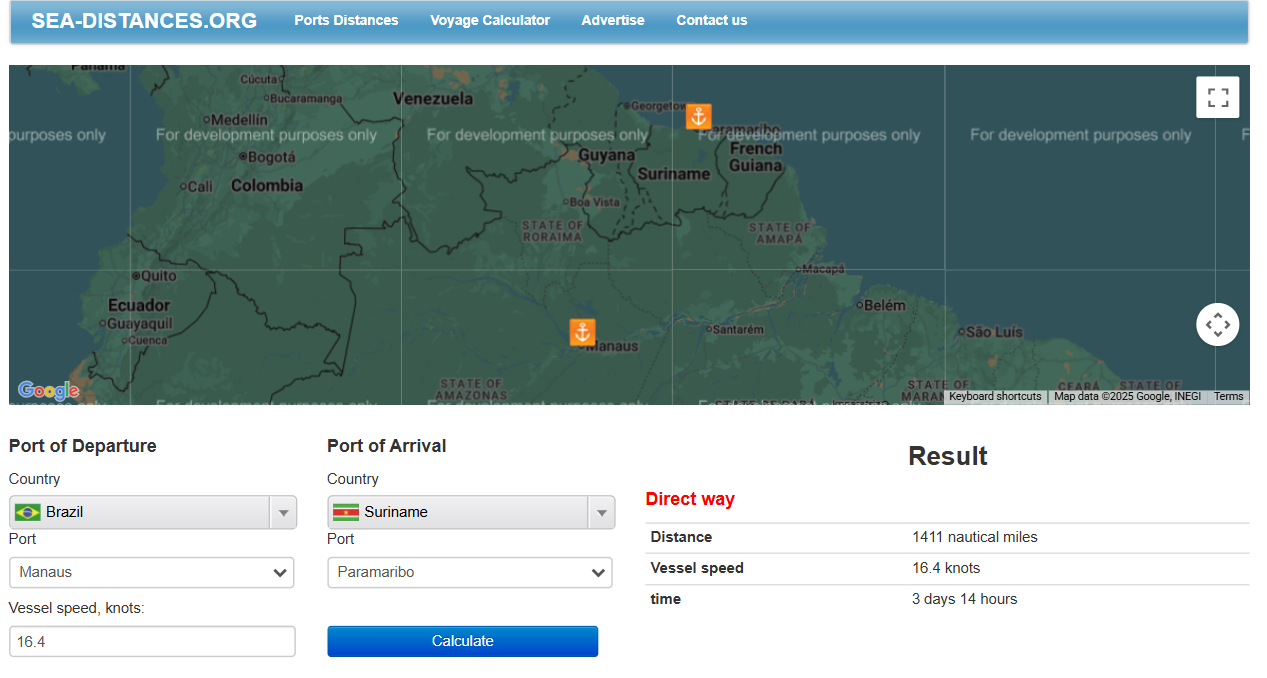
\includegraphics[width=2.3cm]{logo_meyer.png}\par
  \vspace{2pt}
  \normalsize PT M.E.Y.E.R. Industries\par
  Marine Equipment Yard Engineering \& Repair\par
  \small Haekal Meyer Prasetia\par
  0322040053
} \\
\hline
0 & 2025/06/30 & FOR APPROVAL & HMP & GEK & BM \\
\hline
\textbf{REV.} & \textbf{DATE} & \textbf{DESCRIPTION} & \textbf{PREPARED} & \textbf{CHECKED} & \textbf{APPROVED} \\
\hline
\end{tabular}
\end{center}

\cleardoublepageblank

% ==============================
%  DOCUMENT HISTORY SHEET
% ==============================
% PERBAIKAN: \thispagestyle{empty} dihapus (dikomentari) — pada docx, halaman
% ini SUDAH memakai running header (title block) mulai dari sini. Dengan
% \thispagestyle{empty} dihapus, halaman ini otomatis memakai pagestyle
% global "fancy" yang sudah berisi \hvacrunningheader.
%\thispagestyle{empty}
\begin{center}
\textbf{\normalsize DOCUMENT HISTORY SHEET}
\end{center}

\vspace{1em}
\begin{center}
\footnotesize
\renewcommand{\arraystretch}{1.4}
\begin{tabular}{|p{1.2cm}|p{2.2cm}|p{2.2cm}|p{6.4cm}|}
\hline
\textbf{Rev.} & \textbf{Date} & \textbf{Name} & \textbf{Description} \\
\hline
\textit{1} & \textit{12-12-2025} & \textit{GEK} & \textit{Issued for Approval Design of General Arrangement} \\
\hline
\textit{2} & \textit{19-12-2025} & \textit{BM} & \textit{Discussion and approval Standard / Rule} \\
\hline
\textit{3} & \textit{26-12-2025} & \textit{BM \& GEK} & \textit{Assignment of Design \& Calculation} \\
\hline
 & & & \\
\hline
 & & & \\
\hline
 & & & \\
\hline
 & & & \\
\hline
 & & & \\
\hline
 & & & \\
\hline
 & & & \\
\hline
 & & & \\
\hline
 & & & \\
\hline
 & & & \\
\hline
\end{tabular}
\end{center}

\cleardoublepageblank

% ==============================
%  LOG SHEET
% ==============================
% PERBAIKAN: sama seperti Document History Sheet, \thispagestyle{empty}
% dihapus (dikomentari) agar title block header tampil, sesuai docx.
%\thispagestyle{empty}
\begin{center}
\textbf{\normalsize LOG SHEET}\\[4pt]
Air Conditioning \& Ducting Design Project\\[2pt]
\textbf{MT. ANTARES 1}
\end{center}

\vspace{1em}
\begin{center}
\footnotesize
\renewcommand{\arraystretch}{1.4}
\begin{tabular}{|p{0.8cm}|p{5.8cm}|p{1.0cm}|p{1.0cm}|p{3.0cm}|}
\hline
\textbf{NO.} & \textbf{ITEMS} & \textbf{OK.} & \textbf{REV} & \textbf{CHECKED BY (DATE AND SIGN)} \\
\hline
\textit{1} & \textit{Cooling Load Calculation} & $\checkmark$ & & \\
\hline
\textit{2} & \textit{Duct Airflow Calculation} & $\checkmark$ & & \\
\hline
\textit{3} & \textit{Duct Material Selection} & $\checkmark$ & & \\
\hline
\textit{4} & \textit{Duct Sizing and Selection} & $\checkmark$ & & \\
\hline
\textit{5} & \textit{Insulation Material Selection and Thickness Determination} & $\checkmark$ & & \\
\hline
\textit{6} & \textit{Duct Routing} & $\checkmark$ & & \\
\hline
\textit{7} & \textit{Ductswork Drawing (HVAC Duct Layout)} & $\checkmark$ & & \\
\hline
\textit{8} & \textit{Airflow Modeling and Simulation} & $\checkmark$ & & \\
\hline
\textit{9} & \textit{Refrigeration Equipment Layout and Plot Plan} & $\checkmark$ & & \\
\hline
\textit{10} & \textit{Refrigerant Selection} & $\checkmark$ & & \\
\hline
\textit{11} & \textit{Air Handling Unit (AHU) Specification and Selection} & $\checkmark$ & & \\
\hline
\textit{12} & \textit{Airflow Evaluation and Analysis} & $\checkmark$ & & \\
\hline
\textit{13} & \textit{Budget Estimation Plan} & & & \\
\hline
\textit{14} & \textit{Energy Efficiency Assessment} & & & \\
\hline
\textit{15} & \textit{Global Warming Potential (GWP) Assessment} & & & \\
\hline
\textit{16} & \textit{Economic Feasibility Analysis (or Life-Cycle Cost Analysis)} & & & \\
\hline
\textit{17} & \textit{Final Comprehensive Report} & & & \\
\hline
\end{tabular}
\end{center}

\cleardoublepageblank



% ==============================
%  DAFTAR ISI
% \chapter*{DAFTAR ISI}
% ==============================
\tableofcontents
\cleardoublepageblank


% ==============================
%  DAFTAR GAMBAR
% \chapter*{DAFTAR GAMBAR}
% ==============================
\listoffigures
\cleardoublepageblank


% ==============================
%  DAFTAR TABEL
% \chapter*{DAFTAR TABEL}
% ==============================
\listoftables

% ==============================
%  DAFTAR LAMPIRAN
%  \chapter*{DAFTAR LAMPIRAN}
% ==============================
\chapter*{DAFTAR LAMPIRAN}
\addcontentsline{toc}{chapter}{DAFTAR LAMPIRAN}

\noindent Lampiran 1 \quad Gambar Desain General Arrangements (GA) \dotfill 39\\
\noindent Lampiran 2 \quad Spesifikasi Mesin \ldots \dotfill 40

\cleardoublepagekosong



% ==============================
%  KONTEN UTAMA — penomoran arab (1, 2, 3, …)
%  \chapter*{MAINMATTER}
% ==============================
\mainmatter

% =========================================================
%  CHAPTER 1 — INTRODUCTION
% =========================================================
\chapter{INTRODUCTION}

\section{Project Overview}

Kapal M.T. Antares I adalah kapal pengangkut produk minyak (oil products tanker) dengan panjang keseluruhan sekitar 179,88 meter dan lebar sekitar 32,20 meter, berbendera Liberia dan dibangun pada tahun 2008. Kapal ini memiliki daya angkut mati (deadweight) sekitar 45.997 ton serta tonase bruto terdaftar sebesar 28.049. Dalam proyek ini, fokus penelitian akan diarahkan pada sistem pengkondisian udara ruang akomodasi awak kapal, dengan mempertimbangkan kondisi lingkungan laut, beban termal dari peralatan mesin, serta syarat kenyamanan suhu dan kelembapan sesuai standar. Ruang akomodasi menjadi area penting karena awak kapal akan menempatinya dalam durasi panjang selama pelayaran, sehingga sistem HVAC (pemanasan, ventilasi, dan pendingin udara) harus dirancang agar efisien, andal, dan mampu menjaga kualitas udara ideal di tengah kondisi ekstrem di laut.

\textit{Air Handling Unit} (AHU) adalah bagian dari system HVAC yang berguna untuk mengkondisikan dan mensirkulasi udara disuatu ruangan, tepatnya untuk MV ALAHAS. AHU dirancang dan dibuat khusus untuk pengkondisian udara luar agar sesuai dengan ruangan sehubungan dengan suhu, kelembaban dan kebersihan. AHU akan mengambil udara luar, mengkondisikan ulang dan meyalurkannya sebagai udara segar ke dalam ruangan, sehingga akan menghasilkan kualitas udara yang baik. Apabila suhu ruangan panas maka udara segar akan dipanaskan oleh unit pemulihan atau koil pemanas. Sedangkan apabila suhu ruangan dingin maka udara akan didinginkan oleh koil pendingin.

\begin{figure}[H]
\centering
\imgplaceholder[10cm]{5.5cm}{Gambar Air Handling Unit}
\caption{Gambar Air Handling Unit}
\label{fig:ahu}
\end{figure}

\noindent Sumber : (air-handling-units-Indiamart.com)

\section{Scope of Works}

Tuliskan ruang lingkup pekerjaan di sini termasukan permasalahan, tujuan pekerjaan dst. Scope of work disusun berurutan sesuai urutan pekerjaan:

\begin{itemize}
  \item Pemilihan material dan ketebalan insulasi ruangan
  \item Kalkulasi beban pada ruangan yang dilakukan pengkondisian udara.
  \item Kalkulasi dan pemilihan material ducting dan perlengkapan saluran udara.
  \item Kalkulasi dan pemilihan spesifikasi sistem air handling unit.
\end{itemize}

\section{Basic Theory}

Air Handling Unit (AHU) merupakan komponen utama dalam sistem pendingin udara (HVAC) kapal yang berfungsi untuk mengatur, mengondisikan, dan mendistribusikan udara ke seluruh ruangan. AHU bekerja dengan cara mencampur udara luar (fresh air) dan udara balik (return air), kemudian melewatkannya melalui filter, cooling coil, serta fan sebelum dialirkan ke ruang-ruang melalui ducting. Peran AHU sangat penting karena menentukan kenyamanan termal, kualitas udara dalam ruang, serta efisiensi energi sistem pendingin udara di kapal. Dalam perencanaan sistem, perhitungan kapasitas AHU harus didasarkan pada beban pendinginan total ruangan yang meliputi beban sensibel (perubahan suhu udara) dan beban laten (kelembapan udara).

Secara umum, kapasitas AHU dihitung menggunakan persamaan:

\begin{equation}
Q_{total} = \dot{m} \left( h_{in} - h_{out} \right)
\end{equation}

di mana $Q_{total}$ adalah total kapasitas pendinginan (Watt), $\dot{m}$ adalah laju aliran massa udara (kg/s), sedangkan $h_{in}$ dan $h_{out}$ adalah entalpi udara masuk dan keluar koil pendingin (kJ/kg). Untuk menentukan laju aliran udara yang dibutuhkan AHU digunakan formula:

\begin{equation}
V = \dfrac{Q_s}{\rho \, c_p \, \Delta T}
\end{equation}

dengan $V$ adalah laju aliran volumetrik udara (m$^3$/s), $\rho$ adalah densitas udara (1,2 kg/m$^3$), $c_p$ adalah kapasitas panas udara (1005 J/kg$\cdot$K), dan $\Delta T$ adalah perbedaan suhu udara sebelum dan sesudah melewati koil. Selain itu, perhitungan daya fan pada AHU juga perlu dilakukan untuk memastikan udara dapat didorong melalui sistem ducting dengan tekanan yang cukup, menggunakan persamaan:

\begin{equation}
P_{fan} = \dfrac{V \, \Delta p}{\eta_{fan}}
\end{equation}

di mana $P_{fan}$ adalah daya fan (Watt), $\Delta p$ adalah total kehilangan tekanan pada sistem duct (Pa), dan $\eta_{fan}$ adalah efisiensi fan. Dengan demikian, seluruh perencanaan AHU bertujuan agar udara yang dihasilkan memiliki temperatur dan kelembapan sesuai standar kenyamanan serta mampu menjangkau seluruh ruang kapal secara merata dan efisien.

Persamaan-persamaan di atas mengacu pada prinsip dasar mekanika fluida dan termodinamika \citep{cengel2018}, sedangkan prosedur dan koefisien perhitungan beban HVAC mengikuti pedoman \citet{ashrae2018}. Perhitungan numerik yang lebih kompleks pada tahap desain dapat pula dibantu dengan perangkat lunak Engineering Equation Solver (EES) \citep{kleinnellis2014}.


% =========================================================
%  CHAPTER 2 — REFERENCES
% =========================================================
\chapter{REFERENCES}

Sumber referensi dapat menggunakan sumber berikut :

\medskip
\noindent\textbf{Codes}

\noindent Tuliskan code yang digunakan dalam desain (jika tidak ada dapat dihapus).

\medskip
\noindent\textbf{Standards}

\begin{itemize}
  \item ASHRAE
  \item Handbook Of Air Conditioning System Design
  \item Marine Engineering Handbook by R.L Harrington
  \item SNAME 4-7 2007
  \item SNAME 4-16 2015
\end{itemize}

\medskip
\noindent\textbf{Technical documentation of the assets}

\begin{itemize}
  \item \textit{General Arrangement} M.T ANTARES 1
  \item Hasil kalkulasi beban panas setiap ruangan M.T ANTARES 1
\end{itemize}

\medskip
\noindent\textbf{Other references}

\noindent Tuliskan referensi-referensi lain seperti buku-buku atau jurnal paper di sini, dengan menggunakan software Mendeley (bisa download di \url{https://www.mendeley.com/download-reference-manager/windows} dan daftar dgn email @ppns) atau dengan software alternatif Zotero \url{https://www.zotero.org/download/}

\medskip
\noindent Hasil seperti dibawah ini dan tampil secara otomatis :

\nocite{*}
\bibliography{references}


% =========================================================
%  CHAPTER 3 — DESIGN BASIS
% =========================================================
\chapter{DESIGN BASIS}

\section{Principal Dimension}

Kapal yang akan dilakukan kalkulasi desain ini bernama M.T. Antares I. Kapal ini merupakan kapal niaga dengan jenis curah cair (oil product tanker) yang digunakan untuk mengangkut berbagai produk olahan minyak bumi atau bahan bakar cair. Kapal ini memiliki panjang keseluruhan sekitar 179,88 meter, lebar 32,20 meter, dengan daya angkut mati sebesar 45.997 ton, serta berbendera Liberia. Kapal ini dirancang untuk berlayar di perairan internasional, melayani distribusi produk minyak antar pelabuhan niaga. Adapun data utama kapal ini disajikan sebagai berikut.

\begin{table}[H]
\centering
\caption{Principal Dimension}
\begin{tabular}{|c|l|c|c|}
\hline
\rowcolor{tableheader}
\textbf{No.} & \textbf{Parameter} & \textbf{Nilai} & \textbf{Satuan} \\
\hline
\textit{1.} & \textit{Length Perpendicular (LPP)} & 172 & Meter \\
\hline
\textit{2.} & \textit{Length Waterline (LWL)} & 178.8 & Meter \\
\hline
\textit{3.} & \textit{Breadth (B)} & 32.2 & Meter \\
\hline
\textit{4.} & \textit{Height (H)} & 18.7 & Meter \\
\hline
\textit{5.} & \textit{Draft (T)} & 12.072 & Meter \\
\hline
\textit{6.} & \textit{Coefficient Block (CB)} & 0.726 & \\
\hline
\textit{7.} & \textit{Coefficient Midship (Cm)} & 0.986 & \\
\hline
\textit{8.} & \textit{Coefficient Prismatic (CP)} & 0.734 & \\
\hline
\textit{9.} & \textit{Kecepatan (vs)} & 16.4 & \textit{Knot} \\
\hline
\textit{10.} & \textit{Radius Pelayaran} & 1411 & \textit{Nautical Mills} \\
\hline
\textit{11} & \textit{Jumlah ABK} & 34 & \textit{Orang} \\
\hline
\end{tabular}
\end{table}

\section{Sailing Route}

\begin{figure}[H]
\centering
\imgplaceholder[10cm]{6cm}{Sailing Route}
\caption{\textit{Sailing Route}}
\label{fig:sailingroute}
\end{figure}

\section{List of Room}

Dalam mengondisikan udara pada ruang akomodasi di kapal, tentunya untuk mendapatkan perhitungan yang presisi perlu untuk mengetahui jumlah dan jenis ruangan yang udaranya akan dikondisikan. Pada perencanaan kali ini terdapat total 42 ruangan yang akan dikondisikan, dengan masing-masing 14 ruang di main deck, 9 ruang di poop deck, 8 ruang di boat deck, 6 ruang di bridge deck, dan ruang di navigation deck. Adapun tidak semua ruang pada kapal dilakukan pengkondisian udara. Karena juga terdapat ruang yang memang secara aturan tidak perlu atau bahkan dilarang untuk dilakukan pengkondisian udara. Maka dari itu, dibawah ini merupakan data daftar ruang-ruang yang akan dikondisikan pada tiap-tiap \textit{deck} akomodasi yang ada pada kapal.

\subsection*{Main Deck}
\addcontentsline{toc}{subsection}{Main Deck}

\begin{table}[H]
\centering
\caption{Daftar Ruangan yang dikondisikan di \textit{Main Deck}}
\footnotesize
\begin{tabularx}{\textwidth}{|c|c|X|c|c|c|c|c|}
\hline
\rowcolor{tableheader}
\textbf{NO.} & \textbf{DECK} & \textbf{ROOM} & \textbf{P (m)} & \textbf{L (m)} & \textbf{T (m)} & \textbf{A (m2)} & \textbf{V (m3)} \\
\hline
 & \textbf{Main Deck} & & & & & & \\
\hline
1 & & \textit{Mess Room} & 5.6 & 10.5 & 2.5 & \textbf{58.8} & \textbf{147} \\
\hline
2 & & \textit{Seaman (in Room 3 Person)} & 4.8 & 10.5 & 2.5 & \textbf{50.4} & \textbf{126} \\
\hline
3 & & \textit{Fireman (in Room 3 Person)} & 4.8 & 10.5 & 2.5 & \textbf{50.4} & \textbf{126} \\
\hline
4 & & \textit{Oilerman (in Room 3 Person)} & 4.8 & 10.5 & 2.5 & \textbf{50.4} & \textbf{126} \\
\hline
5 & & \textit{Pumpman (in Room 4 Person)} & 4.8 & 10.5 & 2.5 & \textbf{50.4} & \textbf{126} \\
\hline
6 & & \textit{Steward (in Room 2 person)} & 4.8 & 10.5 & 2.5 & \textbf{50.4} & \textbf{126} \\
\hline
7 & & \textit{Assistant Cook (in Room 2 Person)} & 4.8 & 10.5 & 2.5 & \textbf{50.4} & \textbf{126} \\
\hline
8 & & \textit{Boys (in Room 2 Person)} & 4 & 10.5 & 2.5 & \textbf{42} & \textbf{105} \\
\hline
9 & & \textit{GYM Room} & 8 & 4.46 & 2.5 & \textbf{35.68} & \textbf{89.2} \\
\hline
10 & & \textit{Entertaiment Room} & 4 & 4.38 & 2.5 & \textbf{17.52} & \textbf{43.8} \\
\hline
11 & & \textit{Clinic Room} & 5.4 & 4.38 & 2.5 & \textbf{23.652} & \textbf{59.13} \\
\hline
12 & & \textit{Meeting Room} & 7.21 & 9 & 2.5 & \textbf{64.89} & \textbf{162.225} \\
\hline
13 & & \textit{Workshop} & 3.8 & 4.4 & 2.5 & \textbf{16.72} & \textbf{41.8} \\
\hline
14 & & \textit{Prayroom} & 3.2 & 4.4 & 2.5 & \textbf{14.08} & \textbf{35.2} \\
\hline
\end{tabularx}
\end{table}

\subsection*{Poop Deck}
\addcontentsline{toc}{subsection}{Poop Deck}

\begin{table}[H]
\centering
\caption{Daftar Ruangan yang dikondisikan di \textit{Poop Deck}}
\footnotesize
\begin{tabularx}{\textwidth}{|c|c|X|c|c|c|c|c|}
\hline
\rowcolor{tableheader}
 & \multicolumn{2}{c|}{\textbf{Poop Deck}} & & & & & \\
\hline
1 & & \textit{Pray Room} & & 4 & 2.5 & \textbf{26} & \textbf{65} \\
\hline
2 & & \textit{Chief Cook} & & 4 & 2.5 & \textbf{26} & \textbf{65} \\
\hline
3 & & \textit{Boatswain} & & 4.8 & 2.5 & \textbf{31.2} & \textbf{78} \\
\hline
4 & & \textit{Electrician 1} & & 4.8 & 2.5 & \textbf{31.2} & \textbf{78} \\
\hline
5 & & \textit{Electrician 2} & & 4.8 & 2.5 & \textbf{31.2} & \textbf{78} \\
\hline
6 & & \textit{Electrician 3} & & 4.8 & 2.5 & \textbf{31.2} & \textbf{78} \\
\hline
7 & & \textit{Quarter Master} & & 4 & 2.5 & \textbf{26} & \textbf{65} \\
\hline
8 & & \textit{Hospital} & & 4 & 2.5 & \textbf{14.4} & \textbf{36} \\
\hline
9 & & \textit{GYM Room} & & 4 & 2.5 & \textbf{14.4} & \textbf{36} \\
\hline
\end{tabularx}

\vspace{2pt}
{\footnotesize Catatan: kolom L(m) pada baris 1--7 bernilai 6.5 m dan baris 8--9 bernilai 3.6 m sesuai data sumber.}
\end{table}

\subsection*{Boat Deck}
\addcontentsline{toc}{subsection}{Boat Deck}

\begin{table}[H]
\centering
\caption{Daftar Ruangan yang dikondisikan di \textit{Boat Deck}}
\footnotesize
\begin{tabularx}{\textwidth}{|c|X|c|c|c|c|c|}
\hline
\rowcolor{tableheader}
\multicolumn{2}{|c|}{\textbf{Boat Deck}} & & & & & \\
\hline
1 & \textit{Radio Operator 1} & 4.8 & 6.5 & 2.5 & \textbf{31.20} & \textbf{78.00} \\
\hline
2 & \textit{Radio Operator 2} & 4 & 6.5 & 2.5 & \textbf{26.00} & \textbf{65.00} \\
\hline
3 & \textit{Chief Officer (Mualim 1)} & 4.8 & 6.5 & 2.5 & \textbf{31.20} & \textbf{78.00} \\
\hline
4 & \textit{Second Officer (Mualim 2)} & 4.8 & 6.5 & 2.5 & \textbf{31.20} & \textbf{78.00} \\
\hline
5 & \textit{Second Engineer} & 4.8 & 6.5 & 2.5 & \textbf{31.20} & \textbf{78.00} \\
\hline
6 & \textit{Thrith Engineer} & 4.8 & 6.5 & 2.5 & \textbf{31.20} & \textbf{78.00} \\
\hline
7 & \textit{Doctor} & 4 & 6.5 & 2.5 & \textbf{26.00} & \textbf{65.00} \\
\hline
8 & \textit{Workshop} & 3.2 & 6.5 & 2.5 & \textbf{20.80} & \textbf{52.00} \\
\hline
\end{tabularx}
\end{table}

\subsection*{Bridge Deck}
\addcontentsline{toc}{subsection}{Bridge Deck}

\begin{table}[H]
\centering
\caption{Daftar Ruangan yang dikondisikan di \textit{Bridge Deck}}
\footnotesize
\begin{tabularx}{\textwidth}{|c|X|c|c|c|c|c|}
\hline
\rowcolor{tableheader}
\multicolumn{2}{|c|}{\textbf{Bridge Deck}} & & & & & \\
\hline
1 & \textit{Pray Room} & 4 & 6.5 & 2.5 & \textbf{26.00} & \textbf{65.00} \\
\hline
2 & \textit{Captain Day Room} & 3.2 & 6.5 & 2.5 & \textbf{20.80} & \textbf{52.00} \\
\hline
3 & \textit{Captain Room} & 6.4 & 6.5 & 2.5 & \textbf{41.60} & \textbf{104.00} \\
\hline
4 & \textit{Chief Engineer} & 6.4 & 6.5 & 2.5 & \textbf{41.60} & \textbf{104.00} \\
\hline
5 & \textit{Chief Engineer Day Room} & 3.2 & 6.5 & 2.5 & \textbf{20.80} & \textbf{52.00} \\
\hline
6 & \textit{Entertaiment Room} & 4 & 6.5 & 2.5 & \textbf{26.00} & \textbf{65.00} \\
\hline
\end{tabularx}
\end{table}

\subsection*{Navigasi Deck}
\addcontentsline{toc}{subsection}{Navigasi Deck}

\begin{table}[H]
\centering
\caption{Daftar Ruangan yang dikondisikan di \textit{Navigasi Deck}}
\footnotesize
\begin{tabularx}{\textwidth}{|c|X|c|c|c|c|c|}
\hline
\rowcolor{tableheader}
\multicolumn{2}{|c|}{\textbf{Navigation Deck}} & & & & & \\
\hline
1 & \textit{Pray Room} & 1.6 & 5 & 2.5 & \textbf{8} & \textbf{20} \\
\hline
2 & \textit{Chart Room} & 2.4 & 5 & 2.5 & \textbf{12} & \textbf{30} \\
\hline
3 & \textit{Radio Room} & 2.4 & 5 & 2.5 & \textbf{12} & \textbf{30} \\
\hline
4 & \textit{Meeting Room} & 2.4 & 5 & 2.5 & \textbf{12} & \textbf{30} \\
\hline
5 & \textit{Wheel House} & 9.6 & 21 & 2.5 & \textbf{201.6} & \textbf{504} \\
\hline
\end{tabularx}
\end{table}


% =========================================================
%  CHAPTER 4 — METHODOLOGY
% =========================================================
\chapter{METHODOLOGY}

\section{Diagram Alir Pengerjaan}

\begin{figure}[H]
\centering
\begin{tikzpicture}[node distance=0.55cm and 1.2cm, every node/.style={font=\small}]
  \node[startstop] (mulai) {Mulai};
  \node[data, below=of mulai] (studi) {Studi Literatur \& Data};
  \node[data, below=of studi] (data) {Pengumpulan Data Kapal};
  \node[process, below=of data] (beban) {Perhitungan Beban Panas};
  \node[process, below=of beban] (insulasi) {Pemilihan Material \& Ketebalan Insulation};
  \node[process, below=of insulasi] (udara) {Perhitungan Kebutuhan Udara};
  \node[process, below=of udara] (ahu) {Penentuan AHU Room, Service Duct \& Spesifikasi AHU};
  \node[process, below=of ahu] (ducting) {Duct Sizing and Equipment};
  \node[process, below=of ducting] (kalkulasi) {Duct Calculation (Pressure Drop \& Velocity)};
  \node[process, below=of kalkulasi] (rekomendasi) {Recommendation for AHU and Equipment};
  \node[startstop, below=of rekomendasi] (selesai) {Selesai};

  \draw[arrow] (mulai) -- (studi);
  \draw[arrow] (studi) -- (data);
  \draw[arrow] (data) -- (beban);
  \draw[arrow] (beban) -- (insulasi);
  \draw[arrow] (insulasi) -- (udara);
  \draw[arrow] (udara) -- (ahu);
  \draw[arrow] (ahu) -- (ducting);
  \draw[arrow] (ducting) -- (kalkulasi);
  \draw[arrow] (kalkulasi) -- (rekomendasi);
  \draw[arrow] (rekomendasi) -- (selesai);
\end{tikzpicture}
\caption{Diagram Alir Pengerjaan}
\label{fig:flowchart}
\end{figure}

\section{Penjelasan Detail Flowchart}

Flowchart tersebut menggambarkan metodologi pengerjaan proyek perencanaan sistem pendingin udara (Air Handling Unit dan ducting) pada kapal tanker, dengan alur kerja yang sistematis dari tahap awal hingga akhir.

\begin{itemize}
  \item \textbf{Mulai} \\
  Merupakan titik awal dimulainya proyek perencanaan sistem pendingin udara kapal.

  \item \textbf{Studi Literatur \& Data} \\
  Tahap ini meliputi pengumpulan teori dasar tentang prinsip kerja AHU, sistem HVAC di kapal, serta standar yang digunakan seperti IMO, BKI, dan ASHRAE. Tujuannya agar perancangan sistem sesuai regulasi dan prinsip ilmiah.

  \item \textbf{Pengumpulan Data Kapal} \\
  Menghimpun semua data yang diperlukan sebelum melakukan perhitungan teknis, meliputi:
  \begin{itemize}
    \item GA (General Arrangement)
    \item Data kondisi perancangan
    \item Standar perancangan
  \end{itemize}

  \item \textbf{Perhitungan Beban Panas} \\
  Menentukan total beban pendinginan (cooling load) yang harus ditangani oleh sistem tata udara. Perhitungannya mencakup:
  \begin{itemize}
    \item Beban panas transmisi
    \item Beban Panas Penghuni
    \item Beban Panas Jendela
    \item Beban Panas Lampu
    \item Beban Panas Peralatan
    \item Beban Panas Total
  \end{itemize}

  \item \textbf{Pemilihan Material Insulation dan Ketebalan Insulation} --
  Yang sesuai dengan kebutuhan dapat mengurangi beban pendinginan/pemanasan, sehingga konsumsi daya listrik AHU semakin rendah.

  \item \textbf{Perhitungan Kebutuhan Udara} \\
  Menentukan kapasitas udara yang diperlukan untuk menjaga suhu dan kualitas udara ruangan. Perhitungannya meliputi:
  \begin{itemize}
    \item Kapasitas Udara Suplai
    \item Kapasitas Udara Segar
    \item Kapasitas Udara Resirkulasi
  \end{itemize}

  \item \textbf{Penentuan AHU Room, Service Duct dan spesifikasi AHU} \\
  Yang sesuai dengan hasil analisis kebutuhan. Tahap ini juga mencakup pemilihan cooling coil, fan, serta posisi pemasangan AHU di setiap deck agar efisien dan mudah diakses.

  \item \textbf{Duct Sizing and Equipment} \\
  Menentukan ukuran dan tipe ducting (saluran udara) serta memilih peralatan pendukung seperti:
  \begin{itemize}
    \item Diffuser, grille, damper, filter, dan fan.
    \item Ukuran duct dihitung agar laju udara sesuai kecepatan standar dan tidak menimbulkan kebisingan.
  \end{itemize}

  \item \textbf{Duct Calculation (Pressure Drop and Velocity)} \\
  Melakukan perhitungan pressure drop (kehilangan tekanan) dan kecepatan udara dalam duct:
  \begin{itemize}
    \item Pressure drop dipengaruhi oleh panjang duct, belokan (elbow), fitting, dan permukaan saluran.
    \item Hasil perhitungan digunakan untuk menentukan daya fan agar udara tetap mengalir sesuai kebutuhan.
  \end{itemize}

  \item \textbf{Recommendation for AHU and Equipment} \\
  Tahap akhir berupa rekomendasi teknis yang mencakup:
  \begin{itemize}
    \item Kapasitas AHU (dalam CFM atau m$^3$/h).
    \item Jenis fan, filter, dan komponen ducting.
  \end{itemize}

  \item \textbf{Selesai} \\
  Menandai bahwa seluruh proses perancangan sistem tata udara telah selesai dilakukan dan siap untuk tahap implementasi atau evaluasi.
\end{itemize}


% =========================================================
%  CHAPTER 5 — DETAILED CALCULATION & RESULTS
% =========================================================
\chapter{DETAILED CALCULATION \& RESULTS}

Desain sistem pendingin mengacu pada SNAME 4-16 (2005) dimana ada beberapa beban panas yang ditimbulkan yang berpengaruh saat melakukan pengkondisian ruangan. Beberapa beban yang harus diperhitungkan adalah sebagai berikut:

\begin{figure}[H]
\centering
\imgplaceholder[10cm]{6cm}{Beban Panas Ruangan}
\caption{Beban Panas Ruangan}
\label{fig:bebanpanas}
\end{figure}

\section{Perhitungan Beban Panas dan Pemilihan Material Insulation beserta Ketebalan Insulation}

\subsection{Heat Load Transmition}

Beban transmisi adalah aliran panas yang masuk melalui batas (sekat) karena perbedaan suhu di seluruh permukaan batas (sekat).

$\Delta T$ adalah perbedaan suhu di antara ruangan dan suhu ruangan sebelah. Setiap batas atau bagian yang memiliki nilai U atau $\Delta T$ yang berbeda harus dihitung secara terpisah. Jika suhu desain ruangan tidak tersedia, suhu yang tercatat harus digunakan atau perkiraan suhu ruangan bisa dihitung melalui pendekatan neraca panas yang disederhanakan. Nilai U harus merujuk pada versi terbaru dari Laporan Insulasi Termal, Buletin Teknis, dan Penelitian SNAME No. 4-7. Dalam perhitungan beban pendinginan, dampak pendinginan dari ruang tetangga diabaikan kecuali jika suhu yang lebih rendah dipertahankan oleh AC atau peralatan pendinginan. Sementara dalam perhitungan beban pemanasan, panas yang masuk melalui batas dikurangi hanya jika suhu yang lebih tinggi dari ruangan tetangga dijaga oleh sistem pemanas.

\begin{figure}[H]
\centering
\imgplaceholder[10cm]{6cm}{Temperatur Beban Panas}
\caption{Temperatur Beban Panas}
\label{fig:temperaturbebanpanas}
\end{figure}

\subsection{Solar and Transmision Load (Windows)}

Beban transmisi surya + transmisi adalah aliran panas yang masuk akal melalui batas-batas cuaca ruangan yang terpapar matahari. Beban ini merupakan tambahan dari beban transmisi untuk batas atau batas-batas yang terpengaruh, tetapi beban total (surya + transmisi) dihitung dalam satu langkah.

Di mana $\Delta T$ adalah perbedaan antara suhu efektif dan suhu desain ruangan. Nilai U harus sesuai dengan standard SNAME 4-7 pada pemilihan jenis insulasi. Untuk beban solar yang melalui jendela dapat dihitung dengan persamaan yang sesuai.

Jika lebih dari satu batas ruang terpapar sinar matahari, perhitungan perolehan panas yang terpisah harus dilakukan untuk setiap batas atau kombinasi batas dan perolehan simultan terbesar harus digunakan untuk menentukan beban panas matahari dan transmisi. Dimensi yang akan digunakan ketika menghitung area batas, kecuali bahwa area berbayang vertikal tidak boleh disertakan. Area yang diarsir harus dihitung dengan matahari pada sudut 45 dari matahari. Faktor beban matahari yang melalui jendela dan suhu efektif untuk perhitungan tunggal dan multi-batas tercantum dalam Gambar 5.3. Jika suhu desain luar yang berbeda ditentukan, suhu pada Gambar 5.3 harus disesuaikan, ke atas atau ke bawah.

\begin{figure}[H]
\centering
\imgplaceholder[10cm]{6cm}{Glass Solar Factor \& Effective Temperatures}
\caption{Glass Solar Factor \& Effective Temperatures}
\label{fig:glasssolar}
\end{figure}

\subsection{Equipment Load}

Beban peralatan adalah panas sensibel dan laten yang dihasilkan oleh peralatan yang beroperasi di dalam ruang. Untuk ruangan ber-AC, komponen sensibel dan laten dari beban peralatan disertakan. Namun, untuk ruang berventilasi, hanya komponen sensibel yang dimasukkan dalam perhitungan beban pendinginan. Ruang yang biasanya memiliki beban peralatan adalah dapur, pantry, binatu, ruang radio dan komunikasi, ruang kemudi, rumah resistor, kompartemen mesin geladak, dan ruang khusus seperti ruang komputer atau ruang kontrol mesin. Muatan peralatan biasanya akan disertakan untuk ruang tunggu, ruang mess.

Perolehan panas peralatan harus didasarkan pada data pembuangan panas untuk peralatan aktual yang dipasang. Sumber data pembuangan panas terbaik adalah pabrik pembuat peralatan; namun, sering kali peralatan belum dipilih saat perhitungan HVAC dilakukan, dalam hal ini sumber data pembuangan panas lainnya harus digunakan, seperti manual pabrik untuk peralatan serupa atau Buku Panduan Dasar ASHRAE \citep{ashrae2018}. Gambar 5.4 memberikan data pembuangan panas untuk peralatan marine yang umum dan dapat digunakan ketika informasi yang lebih tepat tidak tersedia untuk desain tertentu.

\begin{figure}[H]
\centering
\imgplaceholder[10cm]{6cm}{Equipment Load}
\caption{\textit{Equipment Load}}
\label{fig:equipmentload}
\end{figure}

\subsection{Temperatur Desain Ruangan}

Sistem pengkondisian udara pada ruang akomodasi di M.T Antares 1 yang meliputi main deck, poop deck, boat deck, bridge deck, dan navigation deck akan menggunakan temperatur acuan untuk mendesain seperti pada tabel berikut.

\begin{table}[H]
\centering
\caption{Desain Temperatur}
\begin{tabular}{|l|c|}
\hline
\rowcolor{tableheader}
\textbf{Desain} & \textbf{Temperature (\textdegree F)} \\
\hline
Indoor (Inside Air) Dry Bulb & 78 \\
\hline
Outdoor (Weather Air) Dry Bulb & 95 \\
\hline
Indoor Gangway & 80 \\
\hline
Machinery Space & 130 \\
\hline
Vertical Steel Boundary & 125 \\
\hline
Horizontal Steel Boundary & 145 \\
\hline
\end{tabular}
\end{table}

\subsection{Material Insulation Ruangan}

Guna mendukung kinerja dari sistem pengkondisian udara pada ruang akomodasi di M.T Antares 1 yang meliputi main deck, poop deck, boat deck, bridge deck, dan navigation deck akan menggunakan insulasi untuk ruangan-ruangan tersebut dengan material insulasi dari SNAME. Adapun data heatflow dari SNAME dengan menggunakan material insulasi terdapat sebagai berikut.

\begin{table}[H]
\centering
\caption{Nilai Heat Flow SNAME sesuai Arah Perpindahan Panas}
\begin{tabular}{|c|c|l|c|c|c|}
\hline
\rowcolor{tableheader}
\textbf{Type} & \textbf{Construction} & \textbf{Condition} & \textbf{U} & \textbf{H} & \textbf{D} \\
\hline
\multirow{4}{*}{10} & \multirow{4}{*}{S} & Solar Radiation & --- & .495 & .382 \\
\cline{3-6}
 & & Weather Air to Inside Air & .509 & .425 & .293 \\
\cline{3-6}
 & & Sea Water to Inside Air & --- & .438 & .292 \\
\cline{3-6}
 & & Inside Air to Inside Air & .435 & .361 & .272 \\
\hline
\multirow{4}{*}{55} & \multirow{4}{*}{S} & Solar Radiation & --- & .12 & .11 \\
\cline{3-6}
 & & Weather Air to Inside Air & .11 & .10 & .10 \\
\cline{3-6}
 & & Sea Water to Inside Air & .11 & .11 & .10 \\
\cline{3-6}
 & & Inside Air to Inside Air & .11 & .10 & .10 \\
\hline
\end{tabular}
\end{table}

\section{Hasil Kalkulasi Beban Panas Tiap Ruangan}

\subsection{Main Deck}

\begin{table}[H]
\centering
\caption{Hasil Calculation Beban Panas Tiap Ruangan pada Main Deck}
\begin{tabular}{|c|}
\hline
\textit{(Data perhitungan belum diisi pada dokumen sumber)} \\
\hline
\end{tabular}
\end{table}

\subsection{Poop Deck}

\begin{table}[H]
\centering
\caption{Hasil Calculate Beban Panas Tiap Ruangan pada Poop Deck}
\begin{tabular}{|c|}
\hline
\textit{(Data perhitungan belum diisi pada dokumen sumber)} \\
\hline
\end{tabular}
\end{table}

\subsection{Boat Deck}

\begin{table}[H]
\centering
\caption{Hasil Calculate Beban Panas Tiap Ruangan pada Boat Deck}
\begin{tabular}{|c|}
\hline
\textit{(Data perhitungan belum diisi pada dokumen sumber)} \\
\hline
\end{tabular}
\end{table}

\subsection{Bridge Deck}

\begin{table}[H]
\centering
\caption{Hasil Calculate Beban Panas Tiap Ruangan pada Bridge Deck}
\begin{tabular}{|c|}
\hline
\textit{(Data perhitungan belum diisi pada dokumen sumber)} \\
\hline
\end{tabular}
\end{table}

\subsection{Navigasi Deck}

\begin{table}[H]
\centering
\caption{Hasil Calculate Beban Panas Tiap Ruangan pada Navigasi Deck}
\begin{tabular}{|c|}
\hline
\textit{(Data perhitungan belum diisi pada dokumen sumber)} \\
\hline
\end{tabular}
\end{table}

\section{Hasil Calculate kebutuhan Suplai Udara Tiap Ruangan (Duct Airflow Calculation)}

\subsection{Main Deck}

\begin{table}[H]
\centering
\caption{Hasil Calculate Kebutuhan Suplai Udara Tiap Ruangan pada Main Deck}
\begin{tabular}{|c|}
\hline
\textit{(Data perhitungan belum diisi pada dokumen sumber)} \\
\hline
\end{tabular}
\end{table}

\subsection{Poop Deck}

\begin{table}[H]
\centering
\caption{Haisl Calculate Kebutuhan Suplai Udara Tiap Ruangan pada Poop Deck}
\begin{tabular}{|c|}
\hline
\textit{(Data perhitungan belum diisi pada dokumen sumber)} \\
\hline
\end{tabular}
\end{table}

\subsection{Boat Deck}

\begin{table}[H]
\centering
\caption{Hasil Calculate Kebutuhan Suplai Udara Tiap Ruangan pada Boat Deck}
\begin{tabular}{|c|}
\hline
\textit{(Data perhitungan belum diisi pada dokumen sumber)} \\
\hline
\end{tabular}
\end{table}

\subsection{Bridge Deck}

\begin{table}[H]
\centering
\caption{Hasil Calculate Kebutuhan Suplai Udara Tiap Ruangan pada Bridge Deck}
\begin{tabular}{|c|}
\hline
\textit{(Data perhitungan belum diisi pada dokumen sumber)} \\
\hline
\end{tabular}
\end{table}

\subsection{Navigasi Deck}

\begin{table}[H]
\centering
\caption{Hasil Calculate Kebutuhan Suplai Udara Tiap Ruangan pada Navigasi Deck}
\begin{tabular}{|c|}
\hline
\textit{(Data perhitungan belum diisi pada dokumen sumber)} \\
\hline
\end{tabular}
\end{table}

\section{Duct Material Selection}

\begin{figure}[H]
\centering
\imgplaceholder[10cm]{5cm}{Pemilihan Duct Material}
\caption{Pemilihan \textit{Duct} Material}
\label{fig:ductmaterial}
\end{figure}

\section{DUCT SIZING AND SELECTION}

\subsection{Duct Sizing Branch}

\subsubsection*{Main Deck (Portside Line)}
\begin{figure}[H]
\centering
\imgplaceholder[9cm]{4.5cm}{Duct Sizing Branch Maindeck (Portside Line)}
\caption{\textbf{Duct Sizing Branch Maindeck (Portside Line)}}
\end{figure}

\subsubsection*{Main Deck (Starboard Line)}
\begin{figure}[H]
\centering
\imgplaceholder[9cm]{4.5cm}{Duct Sizing Branch Maindeck (Starboard Line)}
\caption{\textbf{Duct Sizing Branch Maindeck (Starboard Line)}}
\end{figure}

\subsubsection*{Poop Deck (Portside Line)}
\begin{figure}[H]
\centering
\imgplaceholder[9cm]{4.5cm}{Duct Sizing Branch Poopdeck (Portside Line)}
\caption{\textbf{Duct Sizing Branch Poopdeck (Portside Line)}}
\end{figure}

\subsubsection*{Poop Deck (Starboard Line)}
\begin{figure}[H]
\centering
\imgplaceholder[9cm]{4.5cm}{Duct Sizing Branch Poopdeck (Starboard Line)}
\caption{\textbf{Duct Sizing Branch Poopdeck (Starboard Line)}}
\end{figure}

\subsubsection*{Boat Deck (Portside Line)}
\begin{figure}[H]
\centering
\imgplaceholder[9cm]{4.5cm}{Duct Sizing Branch Boatdeck (Portside Line)}
\caption{\textbf{Duct Sizing Branch Boatdeck (Portside Line)}}
\end{figure}

\subsubsection*{Boat Deck (Starboard Line)}
\begin{figure}[H]
\centering
\imgplaceholder[9cm]{4.5cm}{Duct Sizing Branch Boatdeck (Starboard Line)}
\caption{\textbf{Duct Sizing Branch Boatdeck (Starboard Line)}}
\end{figure}

\subsubsection*{Bridge Deck (Portside Line)}
\begin{figure}[H]
\centering
\imgplaceholder[9cm]{4.5cm}{Duct Sizing Branch Bridge Deck (Portside Line)}
\caption{\textbf{Duct Sizing Branch Bridge Deck (Portside Line)}}
\end{figure}

\subsubsection*{Bridge Deck (Starboard Line)}
\begin{figure}[H]
\centering
\imgplaceholder[9cm]{4.5cm}{Duct Sizing Branch Bridge Deck (Starboard Line)}
\caption{\textbf{Duct Sizing Branch Bridge Deck (Starboard Line)}}
\end{figure}

\subsubsection*{Navigasi Deck (Portside Line)}
\begin{figure}[H]
\centering
\imgplaceholder[9cm]{4.5cm}{Duct Sizing Branch Navigasi Deck (Portside Line)}
\caption{\textbf{Duct Sizing Branch Navigasi Deck (Portside Line)}}
\end{figure}

\subsubsection*{Navigasi Deck (Starboard Line)}
\begin{figure}[H]
\centering
\imgplaceholder[9cm]{4.5cm}{Duct Sizing Branch Navigasi Deck (Starboard Line)}
\caption{\textbf{Duct Sizing Branch Navigasi Deck (Starboard Line)}}
\end{figure}

\subsection{Duct Sizing Header (Lower Deck)}
\begin{figure}[H]
\centering
\imgplaceholder[9cm]{4.5cm}{Duct Sizing Header (Lower Deck Line)}
\caption{\textbf{Duct Sizing Header (Lower Deck Line)}}
\end{figure}

\subsection{Duct Sizing Header (Upper Deck)}
\begin{figure}[H]
\centering
\imgplaceholder[9cm]{4.5cm}{Duct Sizing Header (Upper Deck Line)}
\caption{\textbf{Duct Sizing Header (Upper Deck Line)}}
\end{figure}

\section{INSULATION MATERIAL SELECTION AND THICKNESS DETERMINATION}

\textit{(Konten pemilihan material dan penentuan ketebalan insulasi belum diisi pada dokumen sumber.)}

\section{DUCT ROUTING}

\subsubsection*{Main Deck}
\begin{figure}[H]
\centering
\imgplaceholder[9cm]{4.5cm}{Duct Routing Maindeck}
\caption{\textbf{Duct Routing Maindeck}}
\end{figure}

\subsubsection*{Poop Deck}
\begin{figure}[H]
\centering
\imgplaceholder[9cm]{4.5cm}{Duct Routing Poop Deck}
\caption{\textbf{Duct Routing Poop Deck}}
\end{figure}

\subsubsection*{Boat Deck}
\begin{figure}[H]
\centering
\imgplaceholder[9cm]{4.5cm}{Duct Routing Boat Deck}
\caption{\textbf{Duct Routing Boat Deck}}
\end{figure}

\subsubsection*{Bridge Deck}
\begin{figure}[H]
\centering
\imgplaceholder[9cm]{4.5cm}{Duct Routing Bridge Deck}
\caption{\textbf{Duct Routing Bridge Deck}}
\end{figure}

\subsubsection*{Navigasi Deck}
\begin{figure}[H]
\centering
\imgplaceholder[9cm]{4.5cm}{Duct Routing Bridge Deck}
\caption{\textbf{Duct Routing Bridge Deck}}
\end{figure}
% CATATAN: caption "Duct Routing Bridge Deck" pada subsubsection Navigasi Deck
% ditulis persis seperti pada dokumen sumber (kemungkinan salah ketik di
% dokumen asli, seharusnya "Duct Routing Navigasi Deck").

\section{DUCTWORK DRAWING}

\begin{figure}[H]
\centering
\imgplaceholder[10cm]{5.5cm}{Ductwork Drawing}
\caption{\textit{Ductwork Drawing}}
\end{figure}

\section{AIR FLOW MODELLING AND SIMULATION}

\begin{figure}[H]
\centering
\begin{tabular}{cc}
\imgplaceholder[6cm]{4cm}{} & \imgplaceholder[6cm]{4cm}{} \\[4pt]
\imgplaceholder[6cm]{4cm}{} & \imgplaceholder[6cm]{4cm}{} \\
\end{tabular}
\end{figure}

\section{REFRIGERATION EQUIPMENT LAYOUT AND PLOT PLAN}

\begin{figure}[H]
\centering
\imgplaceholder[10cm]{5.5cm}{Layout Ducting}
\caption{\textit{Layout Ducting}}
\end{figure}

\section{REFRIGERANT SELECTION}

\begin{figure}[H]
\centering
\begin{tabular}{cc}
\imgplaceholder[6cm]{4cm}{} & \imgplaceholder[6cm]{4cm}{} \\[4pt]
\imgplaceholder[6cm]{4cm}{} & \imgplaceholder[6cm]{4cm}{} \\
\end{tabular}
\caption{\textit{Refrigerant Selection}}
\end{figure}

GWP adalah singkatan dari global warming potential mengacu pada AR6: sixth assesment report of the IPPC (intergovernmental panel on climate change). GWP adalah potensial setiap 1 Kg refrigerant untuk memanaskan atmosfer tergantung pada setiap 1 Kg karbon dioksida yang terkandung. Berdasarkan tabel perbandingan tiap-tiap refrigerant, maka diketahui bahwa refrigerant type R22 merupakan refrigerant yang paling sesuai digunakan pada sistem ini. Karena memiliki angka GWP yang tidak terlalu tinggi sebesar 1960 mengacu IPPC AR6.

ODP singkatan dari Ozone Depletion Potential, yaitu potensial setiap 1 Kg refrigerant untuk menghancurkan lapisan ozon di atmosfer, tergantung pada setiap 1 Kg Fluorotrichloromethane yang terkandung. Berdasarkan tabel perbandingan tiap-tiap refrigerant, maka diketahui bahwa refrigerant type R22 merupakan refrigerant yang paling sesuai digunakan pada sistem ini. Karena memiliki angka ODP yang tidak tinggi sebesar 0.055, artinya hampir tidak memiliki potensi bahaya ODP.

ISO 817: 2014, mengklasifikasikan refrigerant dalam segi keamanan. ISO 817 menetapkan klasifikasi keamanan refrigerant berdasarkan toxicity (racun) dan flammability (mampu terbakar). Standard ini membagi berdasarkan LFL lower flammable limit, menjadi 3 kelas dengan tambahan sub kelas:

\begin{itemize}
  \item Class 3 : higher flammability
  \item Class 2 : lower flammability
  \item Class 2L : lower burning velocity (BV) class 2s with burning velocities less than or equal to 10 cm/s
  \item Class 1 : no flame propagation
\end{itemize}

Sementara itu klasifikasi toxicity terbagi menjadi 2 kelas berdasarkan paparan:

\begin{itemize}
  \item Class A : (lower chronic toxicity) refrigerant with an occupational exposure limit of 400ppm or greater
  \item Class B : (higher chronic toxicity) refrigerant with an occupational exposure limit of less than 400ppm.
\end{itemize}

Berdasarkan tabel perbandingan tiap-tiap refrigerant, maka diketahui bahwa refrigerant type R22 merupakan refrigerant yang paling sesuai digunakan pada sistem ini. Karena sudah tersertifikasi A1 dari International standard organization (ISO). Secara kelas R22 tidak beracun dan tidak mudah terbakar. Selain itu R22 juga termasuk jenis transitional service refrigerant karena tergolong refrigerant HFC dan chlorin free berdasarkan Structural Classification Of Refrigerants.

\section{AIR HANDLING UNIT (AHU) SPECIFICATION AND SELECTION}

\textit{(Spesifikasi dan seleksi AHU belum diisi pada dokumen sumber.)} Data teknis komponen pendingin (kompresor, cooling coil, dsb.) untuk keperluan spesifikasi dapat merujuk pada katalog produsen, misalnya BITZER \citep{bitzer2022}.

\section{AIRFLOW EVALUATION AND ANALYSIS}

\begin{itemize}
  \item \textbf{Main Deck}
  \item \textbf{Poop Deck}
  \item \textbf{Boat Deck}
  \item \textbf{Bridge Deck}
  \item \textbf{Navigasi Deck}
\end{itemize}

\subsection{Analisa Kebutuhan Suplai Udara pada Ruangan}

Data hasil perhitungan beban panas, laju aliran udara, dan dimensi ducting dari setiap ruangan yang membutuhkan pengkondisian udara disajikan pada tabel berikut :

\begin{table}[H]
\centering
\caption{Hasil Summary calculation AHU tiap Deck}
\begin{tabular}{|c|}
\hline
\textit{(Data perhitungan belum diisi pada dokumen sumber)} \\
\hline
\end{tabular}
\end{table}

\begin{table}[H]
\centering
\caption{Size Main Ducting Yang Didistribusikan}
\begin{tabular}{|c|}
\hline
\textit{(Data perhitungan belum diisi pada dokumen sumber)} \\
\hline
\end{tabular}
\end{table}

\begin{figure}[H]
\centering
\imgplaceholder[9cm]{5cm}{}
\end{figure}

\section{Results and Discussion}

\textit{(Pembahasan hasil belum diisi pada dokumen sumber.)}


% =========================================================
%  CHAPTER 6 — CONCLUSIONS AND RECOMMENDATIONS
% =========================================================
\chapter{CONCLUSIONS and RECOMMENDATIONS}

\section{Conclusions}

Tuliskan kesimpulan di sini untuk menjelaskan hasil pekerjaan mengacu dan menjawab pada scope of work yang sudah dituliskan. Jumlah Kesimpulan mengacu jumlah scope of work yg sudah disusun :

\begin{itemize}
  \item \ldots\ldots\ldots\ldots\ldots.
  \item \ldots\ldots\ldots\ldots\ldots..
  \item \ldots\ldots\ldots\ldots\ldots\ldots\ldots.
\end{itemize}

\section{Recommendations}

Tuliskan rekomendasi-rekomendasi untuk penyempurnaan hasil pekerjaan yg mana rekomendasi itu belum dilakukan atau sebaiknya dilakukan untuk menambah kualitas pekerjaan.


% =========================================================
%  CHAPTER 7 — ATTACHMENT
% =========================================================
\chapter{Attachment}

Cantumkan Lampiran data, gambar-gambar, simulasi dll yang mendukung pada proses pencapaian pekerjaan di scope of work.

\medskip
\noindent Lampiran 1 Gambar Desain General Arrangements (GA)

\noindent \ldots.



% ==============================
% \chapter{DAFTAR PUSTAKA}
%   CATATAN: \bibliography{references} sudah AKTIF dan dipanggil di dalam
%   BAB 2 - REFERENCES (lihat isi \chapter{REFERENCES} di atas), sesuai
%   permintaan agar daftar pustaka tampil di Bab 2, bukan di akhir dokumen.
%   Blok di bawah ini sengaja dibiarkan nonaktif (komentar) sebagai cadangan
%   jika suatu saat daftar pustaka ingin dipindah kembali ke akhir dokumen.
% ==============================
%\titleformat{\chapter}[block]
%  {\centering\bfseries\fontsize{12}{12}\selectfont}
%  {}{}{}
%\titlespacing{\chapter}{0pt}{0pt}{6pt}
%\nocite{*}
%\bibliography{references}

\end{document}